\documentclass[aspectratio=169,10pt]{beamer}

\usetheme{Madrid}
\usecolortheme{seahorse}
\usepackage{amsmath}
\usepackage{booktabs}
\usepackage{graphicx}
\usepackage{tikz}
\usepackage{xcolor}
\usetikzlibrary{arrows.meta,positioning}

\setbeamertemplate{navigation symbols}{}
\setbeamertemplate{footline}{%
  \leavevmode%
  \hbox to \paperwidth{%
    \hfill%
    \scriptsize\insertframenumber{} / \inserttotalframenumber%
    \hspace{1.4em}%
  }%
  \vspace{0.8ex}%
}

\title{SOEN 6011 D2: F6 Beta Function}
\subtitle{From-Scratch Numerical Core, Tkinter GUI, Version Control, and Updated Requirements}
\author{Wei Huang}
\institute{Concordia University}
\date{Summer 2026}

\newcommand{\code}[1]{\texttt{#1}}
\newcommand{\smallcite}[1]{{\scriptsize (#1)}}

\begin{document}

\begin{frame}
  \titlepage
\end{frame}

\begin{frame}{D2 Scope and Dependency Chain}
  \begin{columns}[T]
    \column{0.46\linewidth}
    \begin{block}{D1 baseline}
      \begin{itemize}
        \item Log-gamma identity selected
        \item Python TUI
        \item \code{math.lgamma} and \code{math.exp}
      \end{itemize}
    \end{block}

    \column{0.50\linewidth}
    \begin{block}{D2 increment}
      \begin{enumerate}
        \item \textbf{P5:} implement mathematics from scratch
        \item \textbf{P5:} replace TUI with Tkinter GUI
        \item \textbf{P6:} publish Git repository + README
        \item \textbf{P7:} revise requirements
      \end{enumerate}
    \end{block}
  \end{columns}

  \vspace{0.5em}
  \begin{block}{Interpretation of ``from scratch''}
    No \code{math} module or numerical library. Only input/output, arithmetic,
    exception handling, and Tkinter UI services are used. \smallcite{Kamthan, 2026a}
  \end{block}

  \scriptsize
  D2 revisits the D1 solution and adds new behavior, following an iterative and
  incremental process. \smallcite{Kamthan, 2026b}
\end{frame}

\begin{frame}{P5: From-Scratch Architecture}
\centering
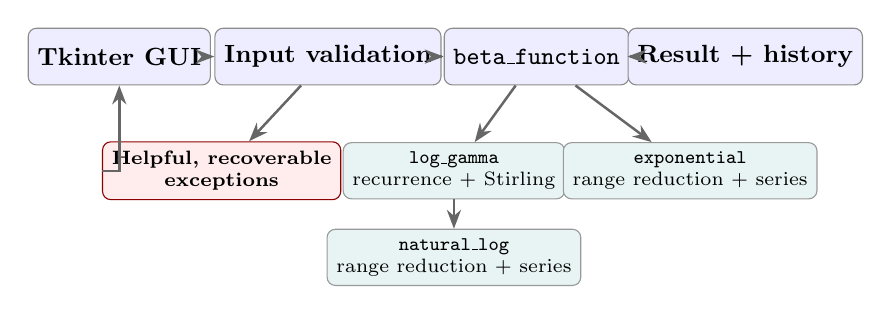
\begin{tikzpicture}[
  node distance=0.65cm and 0.75cm,
  box/.style={rounded corners=3pt, draw=black!45, fill=blue!7,
              minimum width=2.25cm, minimum height=0.72cm,
              align=center, font=\small\bfseries},
  sub/.style={rounded corners=3pt, draw=black!40, fill=teal!9,
              minimum width=2.1cm, minimum height=0.62cm,
              align=center, font=\scriptsize},
  error/.style={rounded corners=3pt, draw=red!55!black, fill=red!7,
                minimum width=2.45cm, minimum height=0.68cm,
                align=center, font=\scriptsize\bfseries},
  arrow/.style={-{Stealth[length=2.4mm]}, line width=0.9pt, draw=black!60}
]
  \node[box] (gui) at (0,0) {Tkinter GUI};
  \node[box] (validation) at (2.65,0) {Input validation};
  \node[box] (beta) at (5.30,0) {\code{beta\_function}};
  \node[box] (result) at (7.95,0) {Result + history};

  \node[error] (errors) at (1.30,-1.45) {Helpful, recoverable\\exceptions};
  \node[sub] (lgamma) at (4.25,-1.45) {\code{log\_gamma}\\recurrence + Stirling};
  \node[sub] (exp) at (7.25,-1.45) {\code{exponential}\\range reduction + series};
  \node[sub] (ln) at (4.25,-2.55) {\code{natural\_log}\\range reduction + series};

  \draw[arrow] (gui) -- (validation);
  \draw[arrow] (validation) -- (beta);
  \draw[arrow] (beta) -- (result);
  \draw[arrow] (beta) -- (lgamma);
  \draw[arrow] (lgamma) -- (ln);
  \draw[arrow] (beta) -- (exp);
  \draw[arrow] (validation) -- (errors);
  \draw[arrow] (errors.west) -| (gui.south);
\end{tikzpicture}

\vspace{0.7em}
\begin{columns}[T]
  \column{0.49\linewidth}
  \begin{block}{Allowed dependencies}
    \small
    \code{tkinter}, \code{ttk}, float parsing, formatting, arithmetic.
  \end{block}
  \column{0.49\linewidth}
  \begin{block}{Prohibited dependencies avoided}
    \small
    No \code{gamma}, \code{lgamma}, \code{log}, \code{exp}, SciPy, or NumPy.
  \end{block}
\end{columns}
\end{frame}

\begin{frame}{P5: Numerical Method and Verification}
  \begin{columns}[T]
    \column{0.48\linewidth}
    \begin{block}{Subordinate mathematics}
      \footnotesize
      \[
        \ln m=2\sum_{k=0}^{\infty}
        \frac{z^{2k+1}}{2k+1},
        \quad z=\frac{m-1}{m+1},\ 1\le m<2
      \]
      \[
        e^r=\sum_{k=0}^{\infty}\frac{r^k}{k!}
      \]
      Shift \(x\) to \(x\ge 8\), then use the Gamma recurrence and a Stirling
      correction series.
      \[
        \log B=\log\Gamma(x)+\log\Gamma(y)-\log\Gamma(x+y)
      \]
    \end{block}

    \column{0.48\linewidth}
    \begin{block}{External verification only}
      \scriptsize
      \begin{tabular}{@{}lll@{}}
        \toprule
        Input & Computed value & Rel. error\\
        \midrule
        \(B(1,1)\) & \(0.999999999999988\) & \(1.24\times10^{-14}\)\\
        \(B(2,3)\) & \(0.0833333333333322\) & \(1.45\times10^{-14}\)\\
        \(B(0.5,0.5)\) & \(3.14159265358979\) & \(1.70\times10^{-15}\)\\
        \(B(100,300)\) & \(5.94745626861\times10^{-99}\) & \(9.40\times10^{-13}\)\\
        \bottomrule
      \end{tabular}
    \end{block}

    \begin{alertblock}{Numeric limit}
      \scriptsize
      A representable finite result is returned; otherwise a
      \code{NumericRangeError} explains overflow or underflow.
    \end{alertblock}
  \end{columns}

  \scriptsize
  Verification used trusted identities and the D1 reference implementation;
  the submitted program itself imports no mathematical library.
  \smallcite{NIST DLMF, 2026a; NIST DLMF, 2026b}
\end{frame}

\begin{frame}{P5: Tkinter GUI and Exception Recovery}
  \begin{columns}[T]
    \column{0.61\linewidth}
    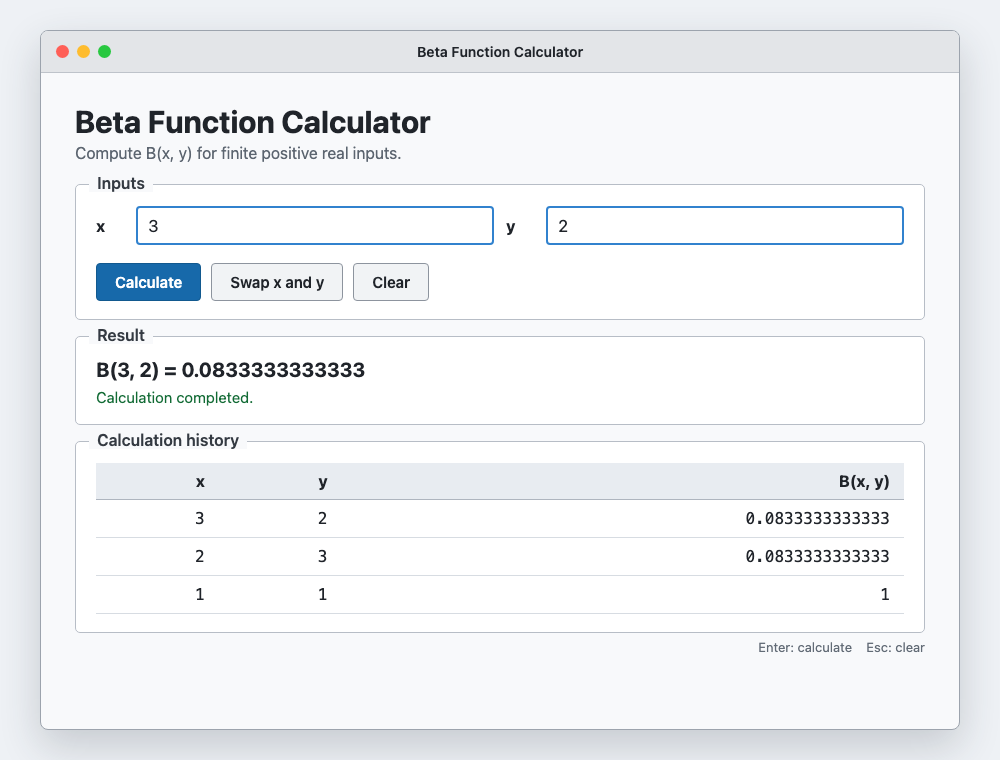
\includegraphics[width=0.98\linewidth]{assets/gui_demo.png}
    \tiny
    GUI demonstration layout reflecting the Tkinter implementation.

    \column{0.35\linewidth}
    \begin{block}{User workflow}
      \scriptsize
      \begin{enumerate}
        \item Enter labeled \(x\) and \(y\)
        \item Calculate or press Enter
        \item Read result and status
        \item Swap, clear, or calculate again
      \end{enumerate}
    \end{block}

    \begin{block}{Helpful exceptions}
      \scriptsize
      \textbf{Missing:} ``x is required.''\\
      \textbf{Nonnumeric:} gives examples.\\
      \textbf{Domain:} names field and \(>0\) rule.\\
      \textbf{Range:} explains unrepresentable result.
    \end{block}

    \begin{block}{Recovery}
      \scriptsize
      Errors update the status area; the window and history remain available.
    \end{block}
  \end{columns}
\end{frame}

\begin{frame}{P6: Distributed Version Control Evidence}
  \begin{columns}[T]
    \column{0.58\linewidth}
    \begin{block}{High-quality local commit history}
      \footnotesize
      \begin{tabular}{@{}lp{5.6cm}@{}}
        \toprule
        Commit & Purpose-focused message\\
        \midrule
        \code{30916e7} & Implement from-scratch Beta numerical core\\
        \code{8d3270f} & Add Tkinter GUI with recoverable input errors\\
        \code{1ba4daa} & Document setup, numerical design, and demo cases\\
        \code{33ed8c8} & Add repository hygiene and GUI demonstration evidence\\
        \bottomrule
      \end{tabular}
    \end{block}

    \column{0.38\linewidth}
    \begin{block}{README coverage}
      \small
      \begin{itemize}
        \item Function and D2 scope
        \item Terminal run command
        \item From-scratch boundary
        \item Demo and error cases
        \item Numerical design and limits
      \end{itemize}
    \end{block}
  \end{columns}

  \vspace{0.4em}
  \begin{alertblock}{Public repository}
    \small
    URL: \textbf{pending authorized GitHub publication}
  \end{alertblock}

  \scriptsize
  Commit logs and README files are lightweight software documentation that make
  decisions and usage explicit. \smallcite{Kamthan, 2026c}
\end{frame}

\begin{frame}{P7: Updated Functional Requirements}
  \scriptsize
  \textbf{Legend:} FR = Functional Requirement. These replace the D1 TUI-focused
  functional requirements.

  \vspace{0.35em}
  \begin{block}{GUI interaction and calculation}
    \footnotesize
    \textbf{D2-FR-01} The system shall provide labeled GUI fields for \(x\) and
    \(y\), plus Calculate, Swap, and Clear commands.\\[0.25em]
    \textbf{D2-FR-02} The system shall accept finite positive real inputs in
    decimal or scientific notation.\\[0.25em]
    \textbf{D2-FR-03} The system shall compute \(B(x,y)\) through the
    from-scratch \code{natural\_log}, \code{exponential}, and
    \code{log\_gamma} operations.\\[0.25em]
    \textbf{D2-FR-04} The system shall display each representable result with
    at least ten significant digits.\\[0.25em]
    \textbf{D2-FR-05} The system shall preserve a history of successful
    calculations during the current session.\\[0.25em]
    \textbf{D2-FR-06} The system shall allow another calculation after a result
    or handled error without restarting.
  \end{block}

  \begin{block}{Why requirements changed}
    \scriptsize
    D1's terminal prompts and quit command were replaced by GUI controls,
    persistent history, and recovery behavior required by P5.
  \end{block}
\end{frame}

\begin{frame}{P7: Updated Constraints and Quality Requirements}
  \begin{columns}[T]
    \column{0.49\linewidth}
    \begin{block}{Constraints}
      \scriptsize
      \textbf{D2-CR-01} The GUI shall use Tkinter.\\[0.25em]
      \textbf{D2-CR-02} The numerical core shall not call built-in or library
      mathematical functions.\\[0.25em]
      \textbf{D2-CR-03} The application shall run from a terminal with
      \code{python3 beta\_function\_gui.py}, independent of an IDE.\\[0.25em]
      \textbf{D2-CR-04} Each handled input error shall name the field and the
      correction needed.
    \end{block}

    \column{0.49\linewidth}
    \begin{block}{Quality requirements}
      \scriptsize
      \textbf{D2-QR-01} Relative error shall be at most \(10^{-10}\) for
      \(B(1,1)=1\) and \(B(2,3)=1/12\); \(B(2,3)\) and \(B(3,2)\) shall agree
      within the same tolerance.\\[0.25em]
      \textbf{D2-QR-02} For \(0<x,y\le1000\) with a representable result, the
      calculation shall complete within 100 ms on the demonstration computer.\\[0.25em]
      \textbf{D2-QR-03} After a handled error, the GUI shall remain open and
      ready for corrected input.
    \end{block}
  \end{columns}

  \vspace{0.35em}
  \scriptsize
  Traceability: P5 architecture satisfies D2-CR-01--04; the verification table
  supports D2-QR-01; GUI recovery supports D2-FR-06 and D2-QR-03.
  \smallcite{ISO/IEC/IEEE, 2018; Kamthan, 2026a}
\end{frame}

\begin{frame}{GAI Use: CASTROFF Evidence for P5--P7}
  \scriptsize
  \begin{columns}[T]
    \column{0.42\linewidth}
    \begin{block}{Tool and CASTROFF}
      \textbf{Tool:} OpenAI ChatGPT/Codex.\\
      \textbf{Context:} SOEN 6011 D2, F6.\\
      \textbf{Audience:} TA and instructor.\\
      \textbf{Style:} concise, evidence-based.\\
      \textbf{Task:} implement and document P5--P7.\\
      \textbf{Role:} software engineering student.\\
      \textbf{Output:} Python, README, requirements, slides.\\
      \textbf{Format:} runnable files and LaTeX.\\
      \textbf{Feedback:} verify mathematically and by execution.
    \end{block}

    \column{0.54\linewidth}
    \begin{block}{Prompt examples and decisions}
      \textbf{P5 prompt:} ``Design Beta from scratch without mathematical
      libraries, including subordinate functions and exceptions.''\\
      \textbf{Revision:} chose recurrence + Stirling, added range checks, and
      rejected direct Gamma multiplication.\\[0.45em]
      \textbf{P6 prompt:} ``Propose purpose-focused commits and a minimal
      README for this scientific GUI.''\\
      \textbf{Accepted after check:} four commits match actual repository
      changes; README commands were executed locally.\\[0.45em]
      \textbf{P7 prompt:} ``Revise D1 shall-statements for the D2 GUI and
      from-scratch constraint.''\\
      \textbf{Revision:} separated functional, constraint, accuracy, timing,
      and recovery requirements.
    \end{block}
  \end{columns}
\end{frame}

\begin{frame}{References}
  \footnotesize
  \begin{list}{}{\setlength{\leftmargin}{0pt}\setlength{\itemsep}{0.5em}}
    \item Kamthan, P. (2026a). \emph{SOEN 6011 Project Description}.
      Concordia University, Summer 2026.
    \item Kamthan, P. (2026b). \emph{Introduction to Software Processes}.
      SOEN 6011 lecture notes.
    \item Kamthan, P. (2026c). \emph{Introduction to Software Engineering
      Documentation}. SOEN 6011 lecture notes.
    \item NIST Digital Library of Mathematical Functions. (2026a).
      Section 5.12, Beta Function, Release 1.2.7.
    \item NIST Digital Library of Mathematical Functions. (2026b).
      Section 5.2, Gamma Function Definitions, Release 1.2.7.
    \item ISO/IEC/IEEE. (2018). \emph{29148:2018 Systems and Software
      Engineering -- Life Cycle Processes -- Requirements Engineering}.
  \end{list}
\end{frame}

\end{document}
